%%%%%%%%%%%%%%%%%%%%%%%%%%%%%%%%%%%%%%%%%
% Beamer Presentation
% LaTeX Template
% Version 1.0 (10/11/12)
%
% This template has been downloaded from:
% http://www.LaTeXTemplates.com
%
% License:
% CC BY-NC-SA 3.0 (http://creativecommons.org/licenses/by-nc-sa/3.0/)
%
%%%%%%%%%%%%%%%%%%%%%%%%%%%%%%%%%%%%%%%%%

%----------------------------------------------------------------------------------------
%	PACKAGES AND THEMES
%----------------------------------------------------------------------------------------

\documentclass{beamer}

\mode<presentation> {
\usetheme{Madrid}
}

\usepackage{graphicx} % Allows including images
\usepackage{booktabs} % Allows the use of \toprule, \midrule and \bottomrule in tables
\usepackage[ngerman]{babel}
\usepackage{fontspec}
%\usepackage{kerkis}            
%\usepackage{kmath} 
\usepackage{pstricks}
%\usepackage{mathtools}
\usepackage{xcolor}
%\usepackage{pifont}
%\usepackage{dsfont}
%\usepackage{marvosym}
%\usepackage{animate}
\usepackage{cancel}
\usepackage{pst-plot}
\usepackage{pst-grad}

\newrgbcolor{ltgray}{0.8 0.8 0.8}
\newrgbcolor{lightred}{1 0.85 0.85}

%----------------------------------------------------------------------------------------
%	TITLE PAGE
%----------------------------------------------------------------------------------------

\title[Akustische Levitation am SFZ SLG]{Forschen am SFZ:\\Akustische Levitation} % The short title appears at the bottom of every slide, the full title is only on the title page

\author[Salomon, Huber, Bienert]{Aaron Salomon, Elias Huber und Marc Bienert} % Your name
\institute[SFZ] % Your institution as it will appear on the bottom of every slide, may be shorthand to save space
{
\parbox[][][c]{1.4cm}{\includegraphics[height=1cm]{SFZ.png}}~\parbox[][][c]{6cm}{\centering Schülerforschungszentrum Südwürttemberg \\ % Your institution for the title page
Standort Bad Saulgau}
}
\date[Uni Ulm, 13.11.18]{\textbf{Kolloquium für Physiklehrende}\\Universität Ulm\\ 13. November 2018} % Date, can be changed to a custom date

\begin{document}

\begin{frame}
\titlepage % Print the title page as the first slide
\end{frame}

\begin{frame}{Die Gravitation spielt mit}
\psset{plotpoints=100}
\begin{columns}
 \begin{column}{0.6\textwidth}

  \begin{center}
   \begin{pspicture}(-3.14,-3.14)(3.14,3.14)
    \psaxes[labels=none,ticks=none]{->}(0,0)(-3.14,-3.14)(3.14,3.14)[$z$,0][$V(x)$,90]
    \psplot[algebraic,linewidth=1pt]{-3.14}{3.14}{sin(x)^2 +(x)*0.6}
    \psplot[algebraic,linecolor=gray,linestyle=dashed]{-3.14}{3.14}{sin(x)^2}
    \psplot[algebraic,linecolor=gray,linestyle=dashed]{-3.14}{3.14}{x}
    \psplot[algebraic,linecolor=orange,linewidth=0.5pt]{-2}{1.35}{-0.09305+0.8*(0.321751+x)^2}
    \rput[rt](2.4,3.2){\parbox{1.3cm}{\footnotesize Gravitations-potential}}
    \rput[rt](3.5,1.4){\parbox{1.3cm}{\footnotesize Akustisches Potential}}
    \rput(1.5,-1.5){
        \begin{pspicture}(-3,-2)(1,2)
         %\psgrid[gridlabels=0,subgridwidth=0.2pt,gridwidth=0.2pt](-2,-2)(2,2)
         \pscircle[fillstyle=solid,fillcolor=white](-1,0){1.7}
         \psaxes[labels=none,ticks=none](0,0)(-2.7,-1.35)(0.7,1.35)
         \pscircle[linecolor=gray,linewidth=0.25pt,fillstyle=gradient,gradbegin=gray,gradend=white,GradientCircle=true](-1.5,0){0.28}
         \pscircle[linecolor=gray,linewidth=0.25pt,fillstyle=gradient,gradbegin=gray,gradend=white,GradientCircle=true](-1.1,0){0.28}
         \pscircle[linecolor=black,linewidth=0.5pt,fillstyle=gradient,gradbegin=black,gradend=gray,GradientCircle=true,GradientScale=1](-1.3,0){0.3}
         \rput{-45}(0.04,-1.34){\psframe[fillstyle=solid,fillcolor=black](0,0)(1,0.5)}
         \psplot[algebraic,linecolor=gray,linestyle=dashed]{-0.8}{0.45}{2*x}
         \psplot[algebraic,linecolor=gray,linestyle=dashed]{-1.7}{0.55}{8*sin(x/4)^2}
         \psplot[algebraic,linewidth=1pt]{-2.7}{0.52}{8*(sin(x/4)^2 +(x/4)*0.6)}
         \psplot[algebraic,linecolor=orange,linewidth=1pt]{-2.7}{0.55}{8*(-0.09305+0.8*(0.321751+x/4)^2)}
         \pscircle[linewidth=1.2pt](-1,0){1.7}
         \psline{<->}(-1.3,-0.744)(-1.3,0)\rput(-0.65,0.5){\footnotesize $z_0$}
         \psline{<->}(-1.3,0.2)(0,0.2)
        \end{pspicture}
    }
   \end{pspicture}
  \end{center}
 \end{column}
 \begin{column}{0.39\textwidth}
 \begin{itemize}
 \item Frequenzmessung:$$ \frac{kV_0}{m}=\sqrt{\frac{\omega^4}{4}+g^2}$$
 \item Abweichungsmessung:$$\frac{kV_0}{m}=\frac{-g}{\sin 2kz}$$
 \end{itemize}
 \end{column}
\end{columns}
\end{frame}

%\bgroup
%canvas}{bg=black}
%\begin{frame}[plain]{}
%\includegraphics[height=\textheighth]{pic/magiclevitation.jpg}\\
%\rput[lt](0,7){\white\Large Levitation}
%\end{frame}
%\egroup
\begin{frame}{Messreihen}

\end{frame}
%\begin{frame}
%\frametitle{Setup}
%\begin{center}
%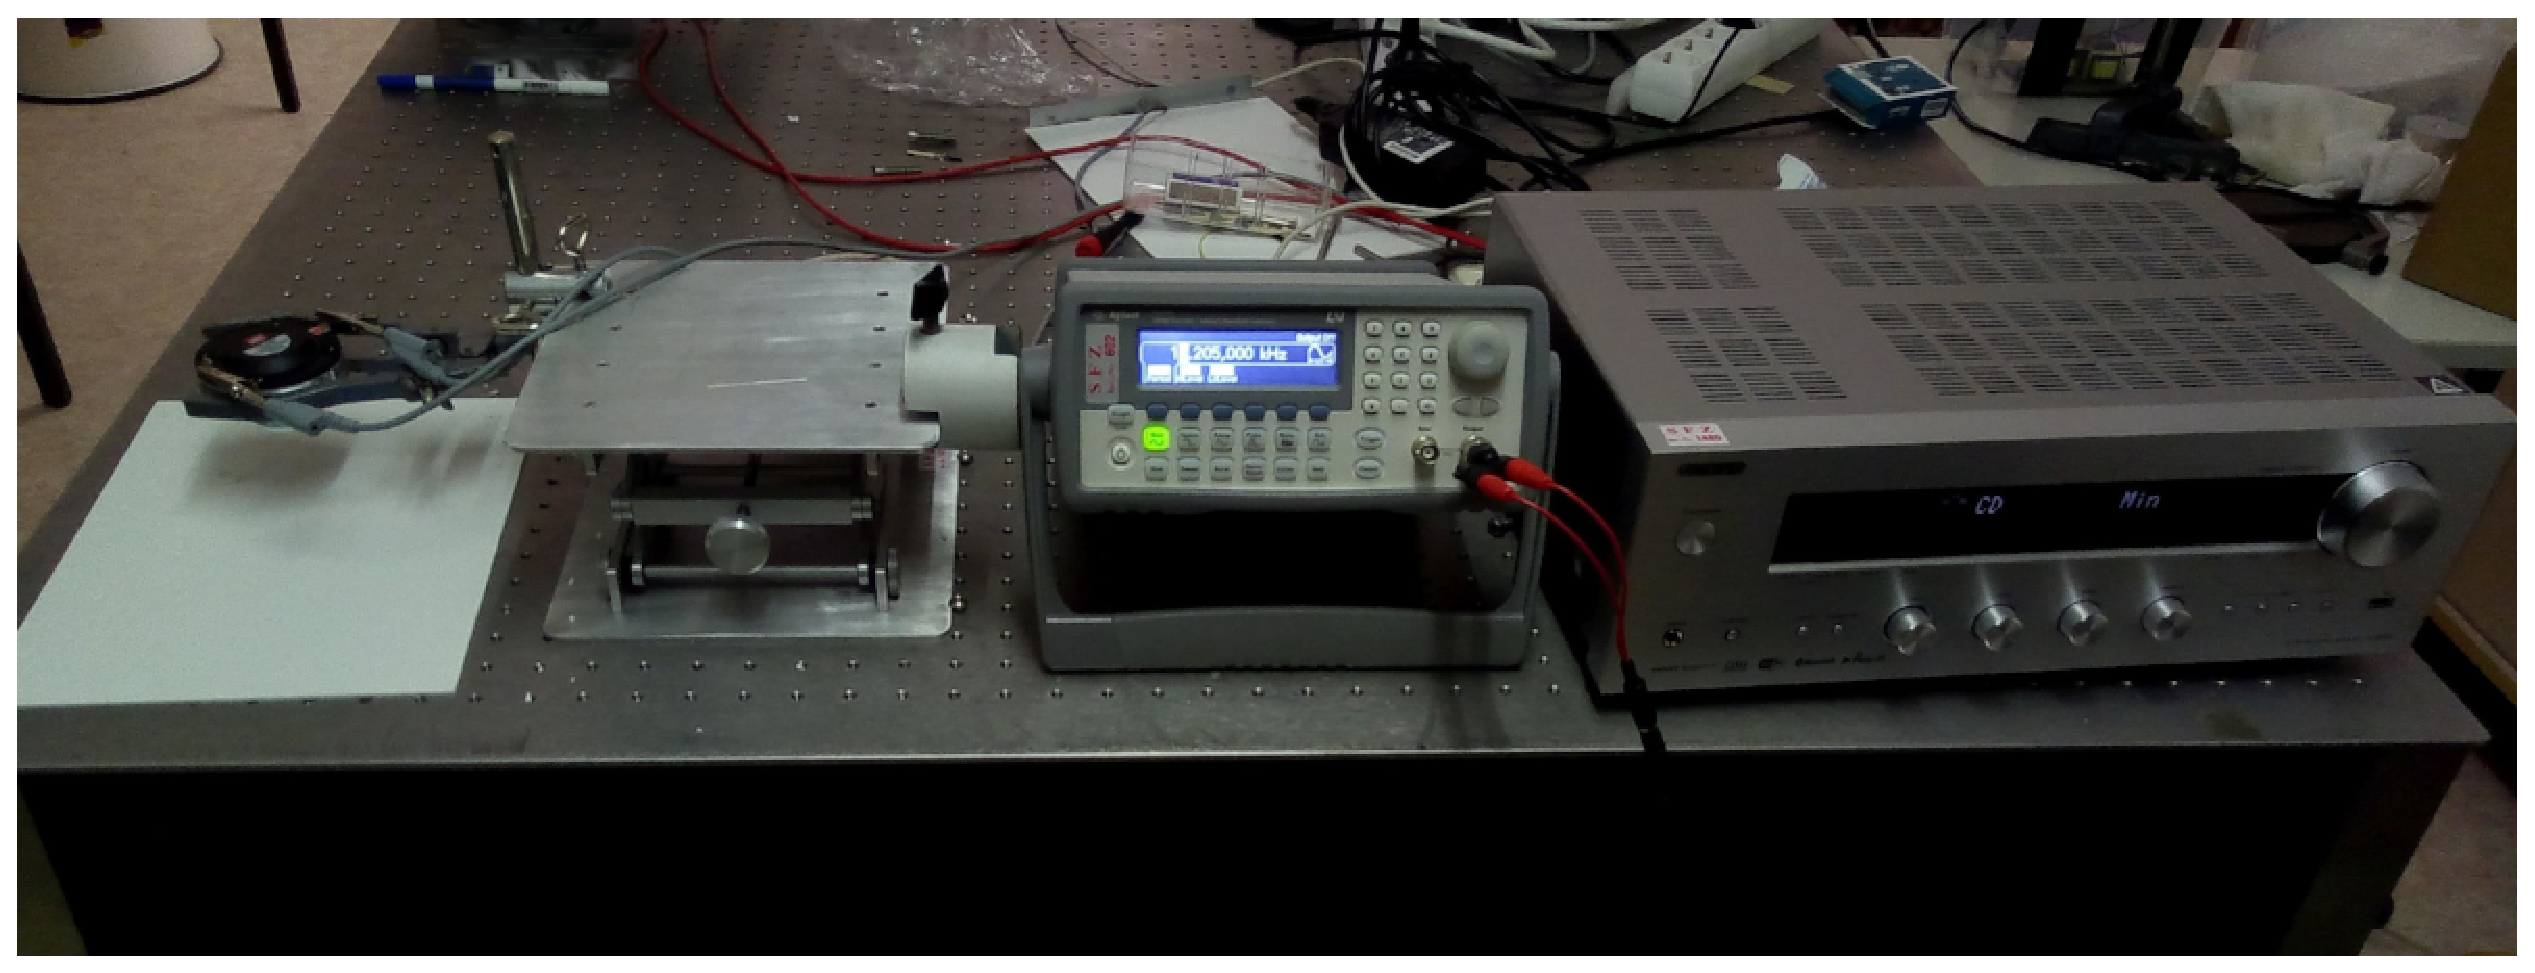
\includegraphics[width=7cm]{BildAufbau}\\
%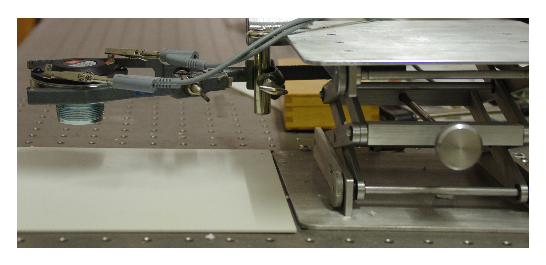
\includegraphics[width=7cm]{Aufbau22}
%\footnotesize{
%\psline{<-}(-1.5,4.6)(0.2,5)\rput(1,5){Amplifier}
%\psline{<-}(-3.5,4.6)(-3,6)\rput(-3,6.2){frequency generator}
%\psline{<-}(-6.5,2)(-7.6,2)\rput(-8.5,2){loudspeaker}}
%\end{center}
%\end{frame}

% \begin{frame}
% \frametitle{Standing wave}
% \begin{minipage}[t]{6cm}
% ~\\
% \animategraphics[scale=0.25,loop]{12}{anim/tmp-}{0}{25}
% \end{minipage}
% \hspace{5mm}
% \begin{minipage}[t]{4cm}
% \begin{itemize}
% \item Incoming wave $\to$ reflected wave
% \item Phase jump of $\pi$
% \item Superposition $\to$ standing wave
% \item Boundary conditions require:\\ Length=$\frac{2n + 1}{4}\lambda$
% \end{itemize}
% \end{minipage}
% \end{frame}

%\begin{frame}
%\frametitle{Pressure and velocity wave}
%\begin{center}
%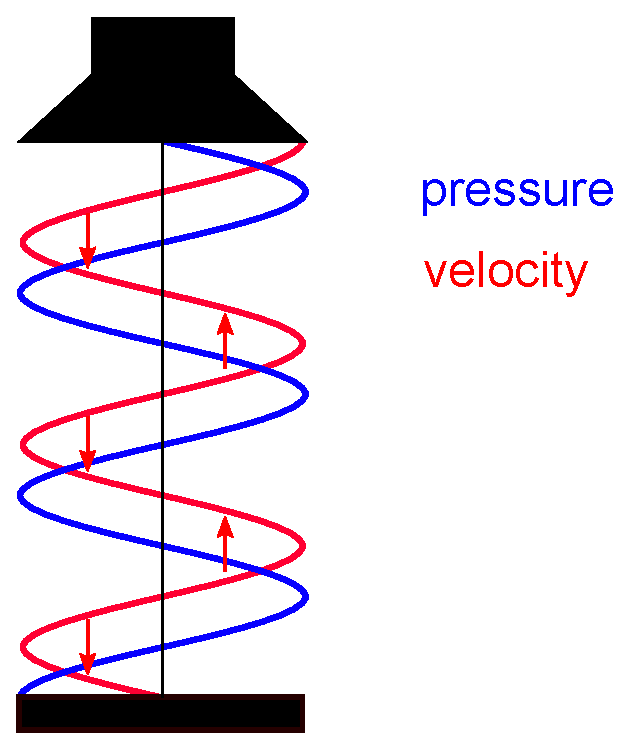
\includegraphics[scale=0.5]{Zeichnungvelocity}
%\end{center}
%\end{frame}

\begin{frame}
\frametitle{Schlieren optics: Setup}
\begin{center}
\includegraphics[scale=0.6]{schlieren_setup_beschriftet}
\end{center}
\end{frame}

\begin{frame}
\frametitle{Schlieren optics: Visualising the acousic field}
\begin{center}
\includegraphics[scale=0.4]{schliere}
\end{center}
\end{frame}

\begin{frame}
\frametitle{Trapping position}
\begin{center}
\includegraphics[scale=0.55]{ZeichnungAbstandsiin}
\end{center}
\begin{align}
\lambda=v_{sound}\cdot f_{speaker}^{-1}=\frac{332\frac{m}{s}}{20000~Hz}=0.0166~m
\end{align}
\end{frame}

\begin{frame}
\frametitle{Scattered Waves}
  \begin{center}
	 \includegraphics{scatwave}
	\end{center}
	\footnotesize{
\psline{<-}(5.5,2.9)(5.5,2.3)\rput(5.5,2.1){monopole wave}
\psline{<-}(8.85,2.9)(8.85,2.3)\rput(8.85,2.1){dipole wave}}
\rput(7.1,6.1){complete wave $=$ incoming wave $+$ scattered waves}
\end{frame}

\begin{frame}
\frametitle{Druckunterschiede bewirken Kraft}
\begin{center}
    \includegraphics[scale=0.8]{inkscape/dichte2}
    
    \psframebox[linecolor=red, fillstyle=solid,fillcolor=lightred]{$F = -  \Delta p \cdot A$}
\end{center}
\end{frame}

\begin{frame}
\frametitle{Impulsflussdichte-Differenz bewirkt Kraft}
\begin{center}
    \begin{pspicture}(-0.5\textwidth,-1cm)(0.5\textwidth,5cm)
   \rput(0,2.5){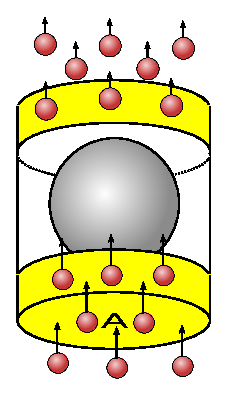
\includegraphics[scale=0.8]{inkscape/impulsfluss.eps}}
   \rput(2.1,1.15){\footnotesize$\left.\rule{0mm}{4mm}\right\} v_1\cdot \Delta t$} % \footnotesize macht die Schriftart kleiner
   \rput(2.1,3.5){\footnotesize$\left.\rule{0mm}{3mm}\right\} v_2\cdot \Delta t$} %<- $-Zeichen schaltet den Mathe-Modus ein (und aus)
   \rput[lt](2.5,0.5){\begin{minipage}{3.5cm}
                \footnotesize
                Einfließender Impuls:
                \vspace{-\abovedisplayskip}%<- normalerweise gibt es einen Abstand zwischen dem Text und der Formel darunter. Der Befehl macht den Abstand rückgängig.
                \begin{flalign*}%<- mathematischer Modus in der flalign-Umgebung
                    p_1 &= (m\, v_1) \cdot (v_1\,\Delta t\, A)\cdot n&\\
                        &= \rho\, v_1^2\cdot A\cdot\Delta t&
                \end{flalign*}
                \end{minipage}
            }
    \rput[lt](2.5,4.75){\begin{minipage}{3.5cm}
                \footnotesize
                Ausfließender Impuls:
                \vspace{-\abovedisplayskip}
                \begin{flalign*}
                    p_2 &= \rho\, v_2^2\cdot A\cdot\Delta t&
                \end{flalign*}
                \end{minipage}
            }
    \psline{-*}(-2,2.5)(0,2.5)
    \rput(-3.3,3){\begin{minipage}{4cm}
                \vspace{-\abovedisplayskip}
                \begin{flalign*}
                   F &= \frac{\Delta p}{\Delta t}&\\
                   &= \left[\rho\, v_2^2 -\rho\, v_1^2\right]\cdot A&
                \end{flalign*}
                \end{minipage}
    }
    \end{pspicture}
    
    \psframebox[linecolor=red, fillstyle=solid,fillcolor=lightred]{$F = \Delta \left[\rho v^2\right]\cdot A$}
\end{center}
%\psset{xuntit=1cm, yunit=1cm)}
%\begin{pspicture} (0,0)(5,5)

%\rput[A](2,0){A}(0,2)
%\end{pspicture}
%\begin{align*}
%&T(x)=\rho v^2\\
   %F &= -A\cdot \left[-T(x) + T(x + dx)\right]\\
	%  &=-A\cdot \left[\frac{-T(x) + T(x + dx)}{dx}dx\right]\\
	%	&=-A\cdot T'(x) dx
%\end{align*}
\end{frame}



%\begin{frame}
%\frametitle{Scattered wave}
%\rput(1.3,0){
 %\begin{minipage}{5cm}
 % \begin{itemize}
 %  \item monopole scattered wave
  % \item dipole scattered wave
   %\end{itemize}
  %end{minipage}
%}
 %\begin{center}
% \includegraphics[scale=0.3]{Zeichnungwave}
% \end{center}
%\end{frame}

%\begin{frame}
%\frametitle{Interference causes the force}
%\begin{align*}
% v= v_{in} + v_{scat}    		
%\end{align*}
%Momentum flux density 
%\begin{align*}
 %  T=\rho v^2 = \rho \left[ \cancel{v_{in}^2} + \cancel{v_{scat}^2} + 2 v_{in} v_{scat} \right]
%\end{align*}
%Locally: $ v_{scat} \sim -v_{in}$\\
%\begin{center}
%\begin{pspicture}(5.5cm,2cm)
   %\psaxes{->}(0cm,0)(5cm,5cm)
	% \psplot[algebraic,linecolor=red]{0}{5}{1+sin(2*x)}
	 %\psplot[algebraic]{0}{5}{1+sin(2*x)^2}
	% \psplot[algebraic,linestyle=dashed]{0}{5}{1-sin(2*x)^2}
	% \psline{->}(-0.25,1)(5.25,1)
	% \psdot(1,1)
	% \psline(1,1)(1,0.17)
	% \psline(1,0.17)(1.25,0.55)
	 %\psline(1,0.17)(0.75,-0.21)
	% \psline[linecolor=blue,linewidth=1.5pt]{->}(1,0.17)(0.25,0.17)\rput(0.7,0.5){\blue $\vec F$}
	% \psdot[dotstyle=o](1,0.17)
	% \rput[l](4.6,0.25){$T_{\rm int}\sim -T$}
	% \rput[l](4.6,1.75){$T\sim v_{\rm in}^2$}
	% \rput[l](5.3,1){$z$}
% \end{pspicture}
%\end{center}
%\end{frame}

\begin{frame}
\frametitle{Potential}
\begin{itemize}
\item Acoustic potential (Phys. Rev. E85 , 016327 (2012))
 \begin{align*}
 %  V(x)= \frac{4\pi}{3} a^3\left[f_1 \frac{1}{2} \kappa_0 (p_0 \sin kx)^2 - f_2 \frac{3}{4} \varrho_0 (v_0 \cos kx)^2 \right]
V(x)&= \frac{4\pi}{3} a^3\left[f_1 \kappa_0 (p_0 \sin kx)^2 - f_2 \varrho_0 (v_0 \cos kx)^2 \right]\\
 \end{align*}
\end{itemize}
\end{frame}

\begin{frame}
\frametitle{Interference causes the force}
Complete velocity field $=$ incoming field $+$ scattered field
\begin{align*}
 v= v_{in} + v_{scat}    		
\end{align*}
Momentum flux density 
\begin{align*}
   T=\rho v^2 = \rho \left[ \cancel{v_{in}^2} + \cancel{v_{scat}^2} + 2 v_{in} v_{scat} \right]
\end{align*}
Locally: $ v_{scat} \sim -v_{in}$
\begin{align*}
T\sim - \rho \cdot v_{in}^2
\end{align*}
\begin{center}
%\includegraphics[scale=0.4]{Zichnungsinableitung}
\end{center}
\end{frame}


\begin{frame}
\frametitle{Approximating the potential}
\begin{align*}V(x)&= \frac{4\pi}{3} a^3\left[f_1 \kappa_0 (p_0 \sin kx)^2 - f_2 \varrho_0 (v_0 \cos kx)^2 \right]\\
    &= V_0\sin^2kx + c
\end{align*}
Taylor-approximation:
$$ V_0\sin^2 kx \approx V_0k^2 x^2 $$
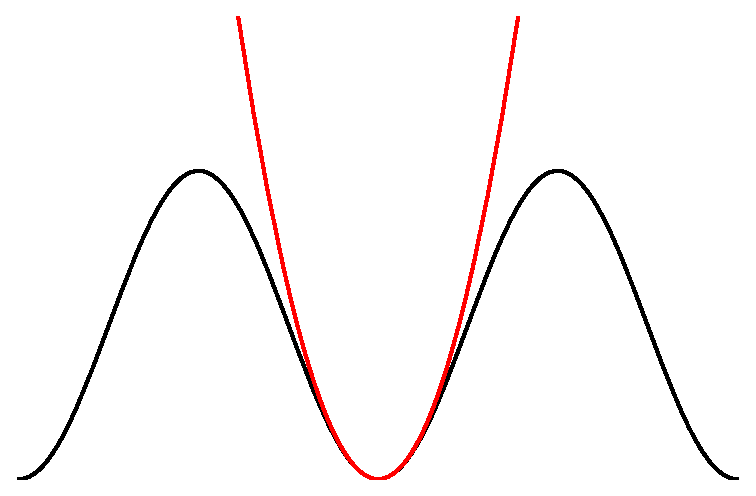
\includegraphics[scale=0.4]{taylor}
\rput(4.2,1.7){
\psframebox{
\begin{minipage}{0.4\textwidth}
\footnotesize
\begin{itemize}
\item Potential of Harmonic Oscillator
\begin{align*}
V(x)= \frac{1}{2} m \omega^2 x^2
\end{align*}
\item Oscillating mass $m$
\item Oscillation frequency $\omega$
\end{itemize}
\end{minipage}}}
\end{frame}

\begin{frame}
\frametitle{Experimental values}
\begin{minipage}{0.595\textwidth}
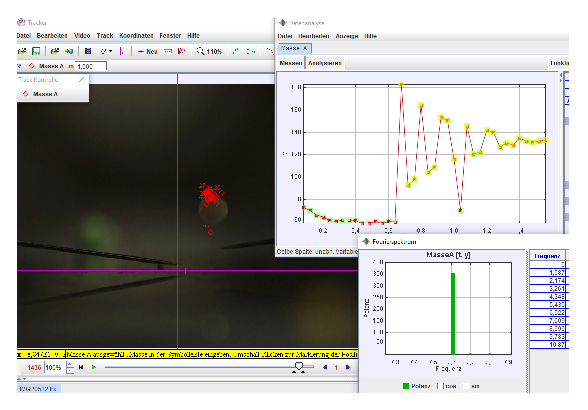
\includegraphics[width=0.99\textwidth]{laengs}
\end{minipage}
\begin{minipage}{0.395\textwidth}
\begin{align*}
 &\frac{1}{2} m \omega^2 \cancel{x^2} = V_o k^2 \cancel{x^2} \\
https://www.overleaf.com/project/5bbf6ec1376b5b41a191881d &m=347\cdot 10^{-9}kg \\ &\omega=(2\pi 7.6)^2\frac{1}{s^2} \\ &k=\left(\frac{2\pi}{0.0221}\frac{1}{m}\right)^2
\end{align*}
\begin{align*}
V_0= 4.895\cdot 10^{-9} J
\end{align*}
\end{minipage}
\end{frame}

\begin{frame}
\frametitle{Force F}
\begin{align*}
 F &= -\frac{d}{dx}(V_0\sin^2kx)\\
   &= -V_0 k \sin kx
\end{align*}
\begin{align*}
 F_{max} &= 4.895\cdot 10^{-9}J \cdot 284.304\frac{1}{m}\\
         &= 1.3916 \cdot 10^{-6}N
\end{align*}
\end{frame}

\begin{frame}
\frametitle{Manipulating the Particle}
\includegraphics[height=4cm]{Auswertung1}
\hspace{1cm}
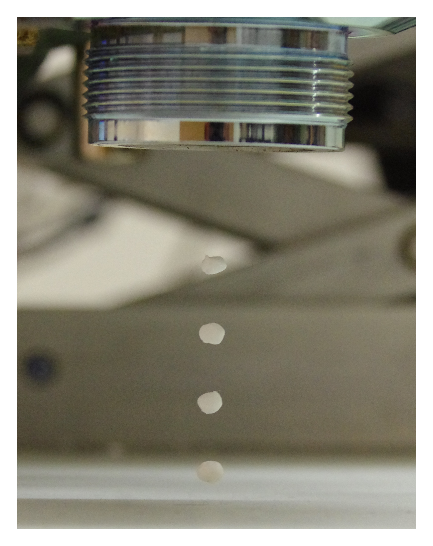
\includegraphics[height=4cm]{Frequenzae}
\end{frame}

\begin{frame}
\frametitle{Manipulating the Particle}
\includegraphics[height=4cm]{Auswertung_angle}
\hspace{1cm}
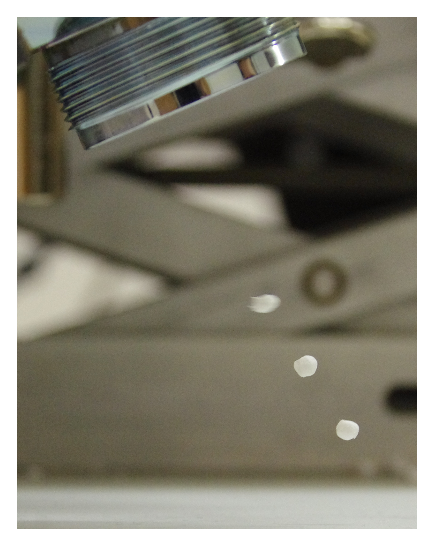
\includegraphics[height=4cm]{Drehung}
\end{frame}

\begin{frame}
\frametitle{Summary}
\begin{itemize}
\item Measurement of the trapping position
\item Wave scattering $\rightarrow$ trapping
\item Measurement of trapping potential
\item Manipulation of the particle
\end{itemize}
\end{frame}

\end{document}